\chapter{Appendix}

This section contains an elementary introduction to reaction-diffusion systems for pattern formation. 

An activator- inhibitor system is described by the following set of equations:

\begin{equation}
\frac{\partial}{\partial t} u(\mathbf{x}, t) = f(u, v) + D_{\text{act}} \nabla^2 u(\mathbf{x}, t)
\end{equation}

\begin{equation}
\frac{\partial}{\partial t} v(\mathbf{x}, t) = g(u, v) + D_{\text{inh}} \nabla^2 v(\mathbf{x}, t)
\end{equation}

where $u(\mathbf{x},\, t)$ is the local density of the activator and $v(\mathbf{x},\, t)$ is the local density of the inhibitor. $D_u$  and $D_v$ are the diffusion coefficients of the ligands or morphogens. The reactions are encoded in the functions $f(u,\,v)$ and $g(u,\,v)$. Various functional forms have been proposed for these functions. Qualitatively, those functions should describe the following facts:
\begin{itemize}
    \item the activator $u$ enhances its own production and the production of the inhibitor $v$;
    \item the inhibitor $v$ suppresses the production of both the activator $u$ and itself,
\end{itemize}
Mathematically, these conditions translate to the following relations on the partial derivatives:
\begin{equation*}
    \begin{cases}
        \frac{\partial f}{\partial u} > 0 \,,\quad \frac{\partial f}{\partial v} < 0 \\
         \frac{\partial g}{\partial u} > 0 \,,\quad \frac{\partial g}{\partial v} < 0 \\       
    \end{cases}
\end{equation*}
It is required that, in absence of diffusion, a uniform stationary state exists, i.e.
$(\overline{u}\,, \overline{v})$
where $f(\overline{u}\,, \overline{v}) = g(\overline{u}\,, \overline{v})=0$. 

$$
\rightarrow
\begin{pmatrix}
  u(\mathbf{x}, t) \\
  v(\mathbf{x}, t) 
\end{pmatrix}
= 
\begin{pmatrix}
  \overline{u} \\
  \overline{v}
\end{pmatrix}
\quad \forall \, \mathbf{x},\, t
$$

Also, it is required that this equilibrium is linearly stable under the effect of small perturbations. Indeed, the key idea of the Turing model is that the instability is driven by diffusion, and appears only above a certain threshold function of the diffusion parameters. 


 The linear stability requirement is satisfied if the jacobian matrix of $F(u,v) = (f(u,v), g(u,v))$ evaluated at the fixed point $(\overline{u}\,, \overline{v})$, $J_F(\overline{u},\, \overline{v})$, has all eigenvalues with negative real parts $\mathcal{R}e(\lambda_i)<0$. Say 
 \begin{equation*}
 		J_{F}(\overline{u}\,, \overline{v}) := \begin{pmatrix}
 			f_u & f_v \\
 			g_u & g_v
 		\end{pmatrix}
 \end{equation*}
Then
$$
Re\{\lambda_i\} <0 \iff 	J_{F}(\overline{u}\,, \overline{v})< 0\quad  \text{(neg. def.)} \iff \begin{cases}
		\text{tr}(J_F) < 0 \\
		\text{det}(J_F)>0
	\end{cases}
	\iff \begin{cases}
		f_u + g_v < 0 \\
		f_u\cdot g_v - f_v\cdot g_u>0
	\end{cases}
$$
Various functional forms for $F(u,v)$ have been proposed. Among the best known:

\begin{itemize}
    \item original Turing (1952) linear functions $f(u,\,v)$:
    \begin{equation}
        \begin{cases}
            f(u,\,v) = a_f\cdot u + b_f\cdot v + c_f \\
            g(u,\,v) = a_g\cdot u + b_g\cdot v + c_g \\            
        \end{cases}
    \end{equation}
    where $a$ coefficients are positive, $b$ coefficients are negative and for $c$, I dont know yet.


    \item the Geiger-Meinhardt (1972) 


\end{itemize}


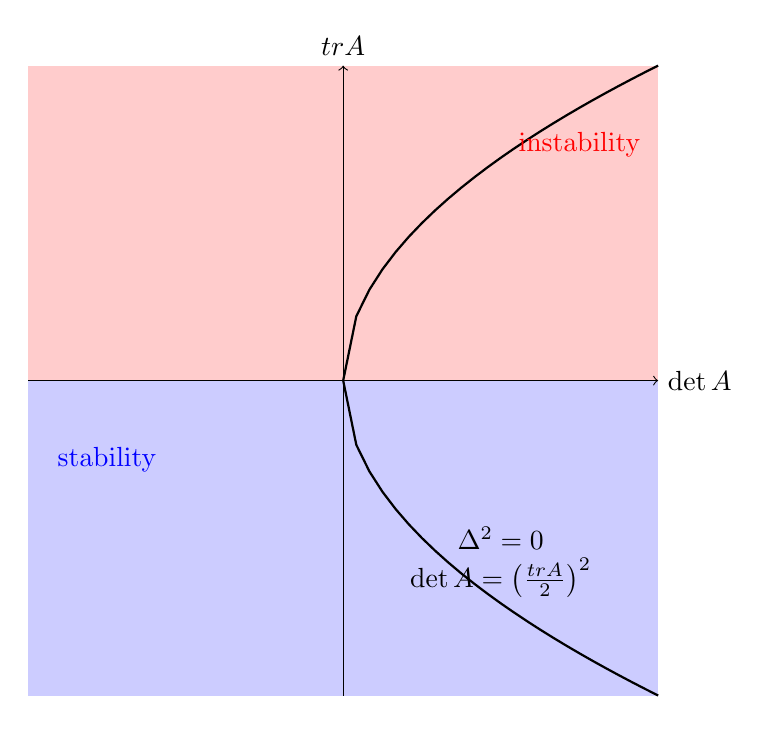
\begin{tikzpicture}
    % Set the size of the grid and the colors
    \fill[red!20] (-4,0) rectangle (4,4);
    \fill[blue!20] (-4,-4) rectangle (4,0);
    
    % Draw the axes
    \draw[->] (-4,0) -- (4,0) node[right] {$\det A$};
    \draw[->] (0,-4) -- (0,4) node[above] {$\operatorname{tr} A$};
    
    % Draw the parabola
    \draw[thick, domain=0:4] plot (\x, {sqrt(\x*4)}) node[right] {};
    \draw[thick, domain=0:4] plot (\x, {-sqrt(\x*4)}) node[right] {};
    
    % Stability and Instability regions
    \node[blue] at (-3,-1) {stability};
    \node[red] at (3,3) {instability};
    
    % Label for the critical point
    \node at (2, -2) {$\Delta^2=0$};
    \node at (2, -2.5) {$\det A = \left(\frac{\operatorname{tr} A}{2}\right)^2$};
\end{tikzpicture}

\citep{murray}


\newpage